%TODO: Formatering
\section{Software}
All sensordata mottas fra microcontrollerene hos en sentral enhet som skal ta seg 
av analyse og visualisering av dataene. Hvordan analysen og visualiseringen av 
dataene skal fungere avhenger av hvilken type sensorer som brukes i systemet. I 
denne rapporten taes det for seg tre forskjellige typer sensorer, strekklapp, 
trykksensor, og vibrasjonssensor. På grunn av likheter i verdier og analysering 
av verdier velger vi å omtale strekklappsensor og trykksensor sammen som 
boltsensor.

\subsection{Analyse av data}
Hvordan data skal analyseres vil være avhengig av hvilken type sensor man velger 
for systemet. 

\subsubsection{Strekklapp/Trykksensor}
Ved bruk av enten strekklapp eller trykksensor vil man få inn en verdi per bolt 
om hvor mye en bolt er strammet til. Analysen vil gå ut på å sammenligne målinger 
med grenseverdier som er satt for de ulike sensorene.

En utfordring ved bruk av strekklapp/trykksensor er håndtering av 
funksjonssvikt i sensor på en bolt. Temperatur og andre eksterne faktorer kan 
også påvirke utslaget i sensorene, så det vil kunne være vanskelig å vite 
nøyaktig hvor løs en bolt egentlig er.

\subsubsection{Vibrasjonssensor}
Ved bruk av vibrasjonssensor vil man få inn verdier fra en sensor som lytter på 
akslingene. Dersom man bruker av en sensor per aksling vil man kunne detektere at 
det er en feil på et av hjulene på akslingen. Ved bruk av to sensorer per aksling 
vil man kunne se hvilket hjul problemet gjelder. Dette kan gjøres ved å se 
hvilken sensor som sendte lyden først.

En kjent feil (f.eks. løse hjulbolter) vil høre til et kjent frekvensområde, som 
kan brukes til å skille ut eventuelle feil som skulle oppstå.

Dersom man kjører på annet underlag slik som snø eller grus, vil dette kunne 
skape problemer med vibrasjonssensor. Frekvensene som mottas fra sensorene vil 
variere etter hvilket underlag man kjører på. Det vil si at frekvensområder for 
kjente feil også bør tilpasses etter underlaget. Dette kan i teorien løses ved å 
enten lagre kjente frekvenseområder for forskjellige underlag. Eventuelt kan man 
sammenligne hver sensor med nåværende gjennomsnitt for alle sensorene for å 
skille ut mulige feil. 

På grunn av uregelmessigheter i veibanen slik som et hull i veien eller flaske 
man kjører på, vil det være nødvendig å klassifisere noe som et problem dersom 
frekvensen som skiller seg ut er gjeldene i mer enn en gitt tid.

\subsection{Visualisering}
Dataene som mottas skal visualiseres etter å ha blitt analysert for å varsle 
sjåfør ved eventuelle problemer. Når det oppstår et problem skal sjåføren bli 
varslet i form av en visuell varsling på et display.

\subsubsection{Strekklapp/Trykksensor}
Sjåføren vil til en hver tid ha mulighet for å se verdiene for de ulike dekkene 
og sensorene. 

Ved bruk av farger kan man visualisere hvor løse mutterne på et hjul er, samt se 
verdier for hver sensor om ønskelig. Dersom man får inn en verdi fra 
strekklappsensor eller trykksensor som er høyere enn en grenseverdien for løse 
muttere, vil man få opp en advarsel på skjermen. Varselen vil variere fra en 
mindre notifikasjon i hjørnet av skjermen for mindre alvorlige feil, til en 
større varsel midt på skjermen for mer alvorlige feil.

En utfordring ved bruk av strekklapp eller trykksensor vil kunne ligge i den 
visuelle representasjonen av feilmeldingen. Det kan i utgangspunktet virke som 
en god idé å vise detaljer ned til hvilken bolt det er registrert avvik i. Det 
som da blir problemet er å vise hvilken posisjon hjulet har rotasjonsmessig for 
å la fører slippe å ettertrekke alle mutre på gitte hjul.

\subsubsection{Vibrasjonssensor}
Visualisering ved bruk av vibrasjonssensorer vil først og fremst være varsling 
ved eventuelle feil som måtte oppstå. Ut i fra om man velger å ha en eller to 
sensorer per aksling vil man få informasjon om hvilket hjul eller aksling 
problemet gjelder. Her vil man også få opp en liten notifikasjon ved mindre 
alvorlige feil og et større varsel ved mer alvorlige feil . Ved å trykke seg 
inn på varselen eller notifikasjonen vil man kunne få en bedre oversikt over 
problemene. Symboler og farger vil vise til hvilke feil som er gjeldene og hvor 
alvorlig det er.

Dersom man bruker vibrasjonssensorer, vil man kun kunne vise hvilket hjul eller 
hjulsett problemet ligger i, og man får ikke en like detaljert oversikt over 
boltene som ved bruk av strekklapp eller trykksensor. Det må også defineres 
en mengde ulike varsler for de ulike typene vibrasjoner som mottas. 
Utfordingen der blir å gi kun akkurat nok informasjon til at varselet blir 
verdifullt, men akkurat lite nok til at det ikke blir forstyrrende og vanskelig 
å forstå hva som formidles.

\subsection{Eksisterende løsninger}
Det eksisterer i skrivende stund ingen softwarebaserte visuelle løsninger dette 
problemet. Bildet under viser hvordan Polyphony Digital løste visualisering av 
dekkslitasje i sitt spill Gran Turismo 6. 
%TODO: Referanse http://s.pro-gmedia.com/videogamer/media/images/ps3/gran_turismo_6/screens/gran_turismo_6_220.jpg, N.P. Web 4. mars
	\newline
		\begin{figure}[H]
			\centering
			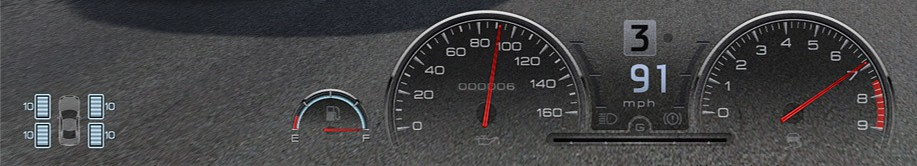
\includegraphics[width=1.00\textwidth]{images/gran-turismo-6-screenshot.jpg}
			\caption{Screenshot fra Gran Turismo 6.}
		\end{figure}
